\documentclass[10pt,a4paper]{article}
\usepackage[margin=18mm,top=22mm,bottom=18mm,headsep=7mm,footskip=9mm]{geometry}
\usepackage{fontspec,amsmath,amssymb,array,tabularx,xcolor,colortbl,tikz,fancyhdr,hyperref}
\usetikzlibrary{arrows.meta}
\setmainfont{NotoSansKR-Regular.ttf}[Path=../../../common/assets/fonts/,BoldFont=NotoSansKR-Semibold.ttf]
\newfontfamily\brandfont{NotoSansKR-Regular.ttf}[Path=../../../common/assets/fonts/,BoldFont=NotoSansKR-Semibold.ttf]
\definecolor{ink}{HTML}{25343D}
\definecolor{accent}{HTML}{216B7A}
\definecolor{muted}{HTML}{637078}
\definecolor{grid}{HTML}{D2DCDF}
\definecolor{soft}{HTML}{F2F6F6}
\definecolor{vectorblue}{HTML}{266CA8}
\definecolor{answerred}{HTML}{C42030}
\newif\ifanswers
\answersfalse
\hypersetup{colorlinks=true,urlcolor=accent,pdftitle={OZ Lab AI Study: Implementing Gradient Descent},pdfauthor={OZ Lab}}
\setlength{\parindent}{0pt}\setlength{\parskip}{2pt}\setlength{\headheight}{21pt}
\setlength{\tabcolsep}{5pt}\renewcommand{\arraystretch}{1.15}\arrayrulecolor{grid}
\pagestyle{fancy}\fancyhf{}
\fancyhead[L]{\brandfont\fontsize{8}{10}\selectfont\bfseries\color{ink}OZ Lab\quad AI Study}
\fancyhead[R]{\brandfont\fontsize{7.5}{10}\selectfont\color{muted}Cost Function / Gradient Descent}
\fancyfoot[L]{\brandfont\fontsize{7}{9}\selectfont\color{muted}MACHINE LEARNING\quad /\quad C1 W1}
\fancyfoot[R]{\brandfont\fontsize{8}{10}\selectfont\color{ink}0\thepage\quad{\color{muted}/\ 04}}
\renewcommand{\headrulewidth}{.3pt}
\renewcommand{\headrule}{\hbox to\headwidth{\color{grid}\leaders\hrule height\headrulewidth\hfill}}
\newcommand{\sect}[2]{\par\vspace{2mm}{\brandfont\fontsize{10}{15}\selectfont\bfseries\color{accent}#1}\quad{\fontsize{14}{19}\selectfont\bfseries\color{ink}#2}\par\vspace{3mm}}
\newcommand{\q}[2]{\par\vspace{3mm}\noindent\makebox[7mm][l]{\brandfont\fontsize{9}{14}\selectfont\bfseries\color{accent}#1}\begin{minipage}[t]{\dimexpr\linewidth-7mm}\fontsize{9.3}{14}\selectfont #2\end{minipage}\par\vspace{1mm}}
\newcommand{\note}[1]{\par\hspace*{7mm}\begin{minipage}{\dimexpr\linewidth-7mm}\fontsize{7.7}{11}\selectfont\color{muted}* #1\end{minipage}\par}
\newcommand{\formula}[1]{\par\vspace{1mm}\begingroup\setlength{\fboxsep}{2.5mm}\colorbox{soft}{\begin{minipage}{\dimexpr\linewidth-5mm}\fontsize{10}{15}\selectfont$\displaystyle #1$\end{minipage}}\endgroup\par\vspace{1mm}}
\newcommand{\given}[1]{\par\vspace{2mm}\hspace*{7mm}{\fontsize{10}{15}\selectfont$\displaystyle #1$}\par\vspace{1mm}}
\newcommand{\ansblank}[2]{\makebox[#1]{\strut\ifanswers\smash{\textcolor{answerred}{\ensuremath{#2}}}\else\textcolor{grid}{\rule{#1}{.3pt}}\fi}}
\newcommand{\cellanswer}[1]{\makebox[0pt]{\ifanswers\textcolor{answerred}{$#1$}\fi}}
\newcommand{\costanswer}[1]{\smash{\makebox[0pt]{\ifanswers\raisebox{-2pt}{\fontsize{7.5}{9}\selectfont\textcolor{answerred}{\shortstack[c]{#1}}}\fi}}}
\newcommand{\strutrow}{\rule[-2.5mm]{0pt}{9mm}}
\newcommand{\solution}[2]{\par\vspace{1.5mm}\begin{minipage}[t][#1][t]{\linewidth}\vspace{0pt}\fontsize{8.3}{12}\selectfont\ifanswers\leavevmode\color{answerred}#2\else{\color{grid}\hrule height .3pt}\fi\end{minipage}\par}
\newcommand{\pick}[3]{{\leavevmode\ifanswers\ifnum#1=#2\color{answerred}\fi\fi$\square$\ #3}}
\newcommand{\choiceprompt}[4]{\par\vspace{2mm}\hspace*{7mm}{\fontsize{8.8}{13}\selectfont\pick{1}{#4}{#1}\qquad\pick{2}{#4}{#2}\qquad\pick{3}{#4}{#3}}\par\vspace{2mm}}
\AtBeginDocument{\fontsize{9.3}{14}\selectfont\color{ink}}
\begin{document}
{\brandfont\fontsize{18}{23}\selectfont\bfseries Implementing Gradient Descent\par}
\vspace{1mm}
{\fontsize{10.5}{15}\selectfont From slope to the next point}\hfill{\ifanswers\color{answerred}\bfseries Worked answers\else\color{muted}Hand-calculation worksheet\fi}\par
\vspace{3mm}{\fontsize{8}{12}\selectfont\color{muted}Name\quad\rule{33mm}{.3pt}\hfill Date\quad\rule{28mm}{.3pt}}\par
\sect{01}{One Update}
\textbf{Shared Data and Model}\par
\vspace{1mm}
\begin{minipage}[t]{.38\linewidth}\vspace{0pt}
\begin{tabularx}{\linewidth}{@{}l*{2}{>{\centering\arraybackslash}X}@{}}
\rowcolor{soft}\strutrow Input $x$ & $-1$ & $1$\\\hline
\strutrow Target $y$ & $-2$ & $2$\\\hline
\end{tabularx}
\end{minipage}\hfill
\begin{minipage}[t]{.57\linewidth}\vspace{0pt}
\formula{f_w(x)=wx\qquad m=2\qquad b=0}
{\fontsize{8}{12}\selectfont\color{muted}Fix $b=0$ and change only $w$\quad One cross-section of the 3D cost surface}
\end{minipage}\par
\q{1}{Calculate the predictions and cost at $w=4$}
\formula{J(w)=\frac1{2m}\sum_{i=1}^{m}\bigl(f_w(x^{(i)})-y^{(i)}\bigr)^2
=\frac{(-w+2)^2+(w-2)^2}{4}=\frac12(w-2)^2}
\begin{minipage}[t]{.47\linewidth}\vspace{2mm}
\given{f_4(-1)=\ansblank{19mm}{-4},\quad f_4(1)=\ansblank{19mm}{4}}
\given{J(4)=\frac{(-4+2)^2+(4-2)^2}{4}=\ansblank{16mm}{2}}
\vspace{2mm}{\fontsize{8}{12}\selectfont\color{muted}Blue point $P$ is $(w,J(w))=(4,2)$}\par
\q{2}{Use the sign of the slope to choose the direction of the update}
\formula{J'(w)=\frac{d}{dw}J(w)=w-2\quad (\alpha>0)}
\end{minipage}\hfill
\begin{minipage}[t]{.49\linewidth}\centering\vspace{0pt}
\begin{tikzpicture}[x=1.0833333333333333cm,y=0.575cm]
\path[use as bounding box] (-0.54,-1.04) rectangle (6.54,9.28);
\draw[grid,line width=.22pt,xstep=1,ystep=1] (0,0) grid (6,8);
\draw[-{Stealth[length=1.7mm]},ink,line width=.5pt] (-0.3,0)--(6.5,0) node[right]{\scriptsize$w$};
\draw[-{Stealth[length=1.7mm]},ink,line width=.5pt] (0,0)--(0,8.72) node[above]{\scriptsize$J(w)$};
\node[below,fill=white,inner sep=.7pt] at (0,0){\scriptsize$0$};
\node[below,fill=white,inner sep=.7pt] at (1,0){\scriptsize$1$};
\node[below,fill=white,inner sep=.7pt] at (2,0){\scriptsize$2$};
\node[below,fill=white,inner sep=.7pt] at (3,0){\scriptsize$3$};
\node[below,fill=white,inner sep=.7pt] at (4,0){\scriptsize$4$};
\node[below,fill=white,inner sep=.7pt] at (5,0){\scriptsize$5$};
\node[below,fill=white,inner sep=.7pt] at (6,0){\scriptsize$6$};
\node[left,fill=white,inner sep=.7pt] at (0,1){\scriptsize$1$};
\node[left,fill=white,inner sep=.7pt] at (0,2){\scriptsize$2$};
\node[left,fill=white,inner sep=.7pt] at (0,3){\scriptsize$3$};
\node[left,fill=white,inner sep=.7pt] at (0,4){\scriptsize$4$};
\node[left,fill=white,inner sep=.7pt] at (0,5){\scriptsize$5$};
\node[left,fill=white,inner sep=.7pt] at (0,6){\scriptsize$6$};
\node[left,fill=white,inner sep=.7pt] at (0,7){\scriptsize$7$};
\node[left,fill=white,inner sep=.7pt] at (0,8){\scriptsize$8$};
\draw[accent,line width=.85pt,domain=0:6,samples=100] plot (\x,{(\x-2)^2/2});
\fill[vectorblue] (4,2.0) circle(2.1pt);
\node[vectorblue,above right,fill=white,inner sep=.8pt] at (4,2.0){\scriptsize$P$};
\ifanswers
\fill[answerred] (3.0,0.5) circle(2.1pt);
\node[answerred,below left,fill=white,inner sep=.8pt] at (3.0,0.5){\scriptsize$Q$};
\fi
\end{tikzpicture}
\end{minipage}\par
\begin{tabularx}{\linewidth}{@{}c c >{\centering\arraybackslash}X@{}}
\rowcolor{soft}\strutrow Current $w$ & Slope $w-2$ & Direction of the next $w$\\\hline
\strutrow $0$ & \ansblank{19mm}{-2} & \pick{1}{2}{Decrease}\quad\pick{2}{2}{Increase}\quad\pick{3}{2}{Unchanged}\\\hline
\strutrow $2$ & \ansblank{19mm}{0} & \pick{1}{3}{Decrease}\quad\pick{2}{3}{Increase}\quad\pick{3}{3}{Unchanged}\\\hline
\strutrow $4$ & \ansblank{19mm}{2} & \pick{1}{1}{Decrease}\quad\pick{2}{1}{Increase}\quad\pick{3}{1}{Unchanged}\\\hline
\end{tabularx}
\q{3}{Starting at $w=4$ with $\alpha=0.5$, make one update and mark the new point $Q$ above}
\formula{w_{k+1}=w_k-\alpha J'(w_k)\qquad \text{current value}\ \longrightarrow\ \text{next value}}
\note{$w_0$ is the starting value; $w_1$ is the first updated value\quad Use the given derivative}
\given{w_{\rm new}=4-0.5\times\ansblank{16mm}{2}=\ansblank{16mm}{3}\qquad J(w_{\rm new})=\ansblank{16mm}{0.5}}
\solution{10mm}{$J'(4)=2>0$, so decrease $w$\quad The cost is lower at $Q=(3,0.5)$\\Calculate the slope at the current $w$, then replace $w$ with the calculated new value}
\vfill
{\fontsize{6.8}{10}\selectfont\color{muted} Reference · Supplied Gradient Descent algorithm and Intuition slides · Update rule and slope signs through C1 W1 slide 65}
\newpage
\sect{02}{Learning Rate A}
\formula{J(w)=\frac12(w-2)^2\qquad J'(w)=w-2\qquad w_0=6\qquad\boxed{\alpha=3}}
\q{4}{Use the same rule to make \textbf{five updates}}
\formula{w_{k+1}=w_k-3(w_k-2)}
\note{Use the last value in a row as the current $w$ in the next row}
\vspace{3mm}
\begingroup\fontsize{8.5}{12}\selectfont\renewcommand{\strutrow}{\rule[-2.5mm]{0pt}{8mm}}
\begin{tabularx}{\linewidth}{@{}c*{4}{>{\centering\arraybackslash}X}@{}}
\rowcolor{soft}\strutrow $k$ & Current $w_k$ & Slope $w_k-2$ & Subtract $\alpha(w_k-2)$ & Next $w_{k+1}$\\\hline
\strutrow 0 & $6$ & \cellanswer{4} & \cellanswer{12} & \cellanswer{-6}\\\hline
\strutrow 1 & \cellanswer{-6} & \cellanswer{-8} & \cellanswer{-24} & \cellanswer{18}\\\hline
\strutrow 2 & \cellanswer{18} & \cellanswer{16} & \cellanswer{48} & \cellanswer{-30}\\\hline
\strutrow 3 & \cellanswer{-30} & \cellanswer{-32} & \cellanswer{-96} & \cellanswer{66}\\\hline
\strutrow 4 & \cellanswer{66} & \cellanswer{64} & \cellanswer{192} & \cellanswer{-126}\\\hline
\end{tabularx}\endgroup
\q{5}{Calculate each cost, plot $P_k=(w_k,J(w_k))$, and draw arrows in order $P_0\to P_1\to\cdots\to P_5$}
\note{$J(w_k)=\frac12(w_k-2)^2$\quad $P_0=(6,8)$}
\vspace{1mm}
\begingroup\fontsize{8}{10}\selectfont
\begin{tabularx}{\linewidth}{@{}*{5}{>{\centering\arraybackslash}X}@{}}
\rowcolor{soft}\rule[-1mm]{0pt}{4.5mm}$J(w_1)$ & $J(w_2)$ & $J(w_3)$ & $J(w_4)$ & $J(w_5)$\\\hline
\rule[-3mm]{0pt}{9mm}\costanswer{$\frac12(-6-2)^2$\\$=32$} & \costanswer{$\frac12(18-2)^2$\\$=128$} & \costanswer{$\frac12(-30-2)^2$\\$=512$} & \costanswer{$\frac12(66-2)^2$\\$=2048$} & \costanswer{$\frac12(-126-2)^2$\\$=8192$}\\\hline
\end{tabularx}\endgroup\par
\vspace{1mm}\begin{minipage}[t]{\linewidth}\centering
\begin{tikzpicture}[x=1cm,y=1cm]
\path[use as bounding box] (-.8,-.55) rectangle (15.4,5.1);
\draw[grid,line width=.22pt] (1.3454545454545455,0)--(1.3454545454545455,4.6);
\node[below,fill=white,inner sep=.7pt] at (1.3454545454545455,0){\scriptsize$-120$};
\draw[grid,line width=.22pt] (4.036363636363636,0)--(4.036363636363636,4.6);
\node[below,fill=white,inner sep=.7pt] at (4.036363636363636,0){\scriptsize$-80$};
\draw[grid,line width=.22pt] (6.7272727272727275,0)--(6.7272727272727275,4.6);
\node[below,fill=white,inner sep=.7pt] at (6.7272727272727275,0){\scriptsize$-40$};
\draw[grid,line width=.22pt] (9.418181818181818,0)--(9.418181818181818,4.6);
\node[below,fill=white,inner sep=.7pt] at (9.418181818181818,0){\scriptsize$0$};
\draw[grid,line width=.22pt] (12.10909090909091,0)--(12.10909090909091,4.6);
\node[below,fill=white,inner sep=.7pt] at (12.10909090909091,0){\scriptsize$40$};
\draw[grid,line width=.22pt] (14.8,0)--(14.8,4.6);
\node[below,fill=white,inner sep=.7pt] at (14.8,0){\scriptsize$80$};
\draw[grid,line width=.22pt] (0,0.92)--(14.8,0.92);
\node[left,fill=white,inner sep=.7pt] at (9.418181818181818,0.92){\scriptsize$2000$};
\draw[grid,line width=.22pt] (0,1.84)--(14.8,1.84);
\node[left,fill=white,inner sep=.7pt] at (9.418181818181818,1.84){\scriptsize$4000$};
\draw[grid,line width=.22pt] (0,2.76)--(14.8,2.76);
\node[left,fill=white,inner sep=.7pt] at (9.418181818181818,2.76){\scriptsize$6000$};
\draw[grid,line width=.22pt] (0,3.68)--(14.8,3.68);
\node[left,fill=white,inner sep=.7pt] at (9.418181818181818,3.68){\scriptsize$8000$};
\draw[grid,line width=.22pt] (0,4.6)--(14.8,4.6);
\node[left,fill=white,inner sep=.7pt] at (9.418181818181818,4.6){\scriptsize$10000$};
\draw[-{Stealth[length=1.7mm]},ink,line width=.5pt] (0,0)--(15.0,0) node[right]{\scriptsize$w$};
\draw[-{Stealth[length=1.7mm]},ink,line width=.5pt] (9.418181818181818,0)--(9.418181818181818,4.8) node[above]{\scriptsize$J(w)$};
\begin{scope}
\clip (0,0) rectangle (14.8,4.6);
\draw[accent,line width=.9pt] plot coordinates {(0.00000,4.63772) (0.14800,4.49513) (0.29600,4.35476) (0.44400,4.21663) (0.59200,4.08072) (0.74000,3.94703) (0.88800,3.81557) (1.03600,3.68634) (1.18400,3.55933) (1.33200,3.43455) (1.48000,3.31200) (1.62800,3.19167) (1.77600,3.07357) (1.92400,2.95770) (2.07200,2.84405) (2.22000,2.73263) (2.36800,2.62344) (2.51600,2.51647) (2.66400,2.41172) (2.81200,2.30921) (2.96000,2.20892) (3.10800,2.11086) (3.25600,2.01502) (3.40400,1.92141) (3.55200,1.83003) (3.70000,1.74087) (3.84800,1.65394) (3.99600,1.56923) (4.14400,1.48676) (4.29200,1.40651) (4.44000,1.32848) (4.58800,1.25268) (4.73600,1.17911) (4.88400,1.10776) (5.03200,1.03864) (5.18000,0.97175) (5.32800,0.90708) (5.47600,0.84464) (5.62400,0.78443) (5.77200,0.72644) (5.92000,0.67068) (6.06800,0.61715) (6.21600,0.56584) (6.36400,0.51675) (6.51200,0.46990) (6.66000,0.42527) (6.80800,0.38287) (6.95600,0.34269) (7.10400,0.30474) (7.25200,0.26902) (7.40000,0.23552) (7.54800,0.20425) (7.69600,0.17520) (7.84400,0.14839) (7.99200,0.12380) (8.14000,0.10143) (8.28800,0.08129) (8.43600,0.06338) (8.58400,0.04769) (8.73200,0.03423) (8.88000,0.02300) (9.02800,0.01399) (9.17600,0.00721) (9.32400,0.00266) (9.47200,0.00033) (9.62000,0.00023) (9.76800,0.00236) (9.91600,0.00671) (10.06400,0.01328) (10.21200,0.02209) (10.36000,0.03312) (10.50800,0.04638) (10.65600,0.06186) (10.80400,0.07957) (10.95200,0.09951) (11.10000,0.12167) (11.24800,0.14606) (11.39600,0.17267) (11.54400,0.20152) (11.69200,0.23259) (11.84000,0.26588) (11.98800,0.30140) (12.13600,0.33915) (12.28400,0.37912) (12.43200,0.42132) (12.58000,0.46575) (12.72800,0.51240) (12.87600,0.56128) (13.02400,0.61239) (13.17200,0.66572) (13.32000,0.72128) (13.46800,0.77907) (13.61600,0.83908) (13.76400,0.90131) (13.91200,0.96578) (14.06000,1.03247) (14.20800,1.10139) (14.35600,1.17253) (14.50400,1.24590) (14.65200,1.32150) (14.80000,1.39932)};
\end{scope}
\fill[vectorblue] (9.82182,0.00368) circle(1.9pt);
\draw[vectorblue,line width=.3pt] (9.82182,0.00368)--(10,.6);
\node[vectorblue,above,fill=white,inner sep=1pt] at (10,.6){\scriptsize$P_0$};
\ifanswers
\draw[-{Stealth[length=1.65mm]},shorten <=2pt,shorten >=2pt,answerred,line width=.8pt] (9.82182,0.00368)--(9.01455,0.01472);
\draw[-{Stealth[length=1.65mm]},shorten <=2pt,shorten >=2pt,answerred,line width=.8pt] (9.01455,0.01472)--(10.62909,0.05888);
\draw[-{Stealth[length=1.65mm]},shorten <=2pt,shorten >=2pt,answerred,line width=.8pt] (10.62909,0.05888)--(7.40000,0.23552);
\draw[-{Stealth[length=1.65mm]},shorten <=2pt,shorten >=2pt,answerred,line width=.8pt] (7.40000,0.23552)--(13.85818,0.94208);
\draw[-{Stealth[length=1.65mm]},shorten <=2pt,shorten >=2pt,answerred,line width=.8pt] (13.85818,0.94208)--(0.94182,3.76832);
\fill[answerred] (9.01455,0.01472) circle(1.6pt);
\draw[answerred,line width=.3pt] (9.01455,0.01472)--(8.7,0.43);
\node[answerred,above,fill=white,inner sep=.7pt] at (8.7,0.5){\scriptsize$P_1$};
\fill[answerred] (10.62909,0.05888) circle(1.6pt);
\draw[answerred,line width=.3pt] (10.62909,0.05888)--(11,0.27999999999999997);
\node[answerred,above,fill=white,inner sep=.7pt] at (11,0.35){\scriptsize$P_2$};
\fill[answerred] (7.40000,0.23552) circle(1.6pt);
\node[answerred,above left,fill=white,inner sep=.7pt] at (7.40000,0.23552){\scriptsize$P_3$};
\fill[answerred] (13.85818,0.94208) circle(1.6pt);
\node[answerred,above right,fill=white,inner sep=.7pt] at (13.85818,0.94208){\scriptsize$P_4$};
\fill[answerred] (0.94182,3.76832) circle(1.6pt);
\node[answerred,above right,fill=white,inner sep=.7pt] at (0.94182,3.76832){\scriptsize$P_5$};
\fi
\end{tikzpicture}
\end{minipage}\par
\q{6}{Check the \textbf{position and cost} after five updates}
\given{w_5=\ansblank{23mm}{-126}\qquad |w_5-2|=\ansblank{23mm}{128}}
\given{J(w_5)=\tfrac12(w_5-2)^2=\ansblank{23mm}{8192}\qquad J(w_0)=8}
\choiceprompt{Closer}{Farther away}{Almost no movement}{2}
Explain why the cost increased even though you moved opposite to the slope
\solution{12mm}{A step is too large: it crosses the minimum and reaches a higher point on the other side\\The distance grows as $4,8,16,32,64,128$, so the sequence diverges}
\newpage
\sect{03}{Learning Rate B}
\formula{J(w)=\frac12(w-2)^2\qquad J'(w)=w-2\qquad w_0=6\qquad\boxed{\alpha=0.01}}
\q{7}{Use the same rule to make \textbf{five updates}}
\formula{w_{k+1}=w_k-0.01(w_k-2)}
\note{For B, round each new $w$ to two decimal places before the next row\quad Table and plot values are approximate}
\vspace{3mm}
\begingroup\fontsize{8.5}{12}\selectfont\renewcommand{\strutrow}{\rule[-2.5mm]{0pt}{8mm}}
\begin{tabularx}{\linewidth}{@{}c*{4}{>{\centering\arraybackslash}X}@{}}
\rowcolor{soft}\strutrow $k$ & Current $w_k$ & Slope $w_k-2$ & Subtract $\alpha(w_k-2)$ & Next $w_{k+1}$\\\hline
\strutrow 0 & $6$ & \cellanswer{4} & \cellanswer{0.04} & \cellanswer{5.96}\\\hline
\strutrow 1 & \cellanswer{5.96} & \cellanswer{3.96} & \cellanswer{0.0396} & \cellanswer{5.92}\\\hline
\strutrow 2 & \cellanswer{5.92} & \cellanswer{3.92} & \cellanswer{0.0392} & \cellanswer{5.88}\\\hline
\strutrow 3 & \cellanswer{5.88} & \cellanswer{3.88} & \cellanswer{0.0388} & \cellanswer{5.84}\\\hline
\strutrow 4 & \cellanswer{5.84} & \cellanswer{3.84} & \cellanswer{0.0384} & \cellanswer{5.8}\\\hline
\end{tabularx}\endgroup
\q{8}{Calculate each cost, plot $P_k=(w_k,J(w_k))$, and draw arrows in order $P_0\to P_1\to\cdots\to P_5$}
\note{$J(w_k)=\frac12(w_k-2)^2$\quad $P_0=(6,8)$}
\vspace{1mm}
\begingroup\fontsize{8}{10}\selectfont
\begin{tabularx}{\linewidth}{@{}*{5}{>{\centering\arraybackslash}X}@{}}
\rowcolor{soft}\rule[-1mm]{0pt}{4.5mm}$J(w_1)$ & $J(w_2)$ & $J(w_3)$ & $J(w_4)$ & $J(w_5)$\\\hline
\rule[-3mm]{0pt}{9mm}\costanswer{$\frac12(5.96-2)^2$\\$=7.8408$} & \costanswer{$\frac12(5.92-2)^2$\\$=7.6832$} & \costanswer{$\frac12(5.88-2)^2$\\$=7.5272$} & \costanswer{$\frac12(5.84-2)^2$\\$=7.3728$} & \costanswer{$\frac12(5.8-2)^2$\\$=7.22$}\\\hline
\end{tabularx}\endgroup\par
\vspace{1mm}\begin{minipage}[t]{\linewidth}\centering
\begin{tikzpicture}[x=1cm,y=1cm]
\path[use as bounding box] (-.8,-.55) rectangle (15.4,5.1);
\draw[grid,line width=.22pt] (0.0,0)--(0.0,4.6);
\node[below,fill=white,inner sep=.7pt] at (0.0,0){\scriptsize$0$};
\draw[grid,line width=.22pt] (2.1764705882352944,0)--(2.1764705882352944,4.6);
\node[below,fill=white,inner sep=.7pt] at (2.1764705882352944,0){\scriptsize$1$};
\draw[grid,line width=.22pt] (4.352941176470589,0)--(4.352941176470589,4.6);
\node[below,fill=white,inner sep=.7pt] at (4.352941176470589,0){\scriptsize$2$};
\draw[grid,line width=.22pt] (6.529411764705883,0)--(6.529411764705883,4.6);
\node[below,fill=white,inner sep=.7pt] at (6.529411764705883,0){\scriptsize$3$};
\draw[grid,line width=.22pt] (8.705882352941178,0)--(8.705882352941178,4.6);
\node[below,fill=white,inner sep=.7pt] at (8.705882352941178,0){\scriptsize$4$};
\draw[grid,line width=.22pt] (10.882352941176471,0)--(10.882352941176471,4.6);
\node[below,fill=white,inner sep=.7pt] at (10.882352941176471,0){\scriptsize$5$};
\draw[grid,line width=.22pt] (13.058823529411766,0)--(13.058823529411766,4.6);
\node[below,fill=white,inner sep=.7pt] at (13.058823529411766,0){\scriptsize$6$};
\draw[grid,line width=.22pt] (0,0.9199999999999999)--(14.8,0.9199999999999999);
\node[left,fill=white,inner sep=.7pt] at (0.0,0.9199999999999999){\scriptsize$2$};
\draw[grid,line width=.22pt] (0,1.8399999999999999)--(14.8,1.8399999999999999);
\node[left,fill=white,inner sep=.7pt] at (0.0,1.8399999999999999){\scriptsize$4$};
\draw[grid,line width=.22pt] (0,2.76)--(14.8,2.76);
\node[left,fill=white,inner sep=.7pt] at (0.0,2.76){\scriptsize$6$};
\draw[grid,line width=.22pt] (0,3.6799999999999997)--(14.8,3.6799999999999997);
\node[left,fill=white,inner sep=.7pt] at (0.0,3.6799999999999997){\scriptsize$8$};
\draw[grid,line width=.22pt] (0,4.6)--(14.8,4.6);
\node[left,fill=white,inner sep=.7pt] at (0.0,4.6){\scriptsize$10$};
\draw[-{Stealth[length=1.7mm]},ink,line width=.5pt] (0,0)--(15.0,0) node[right]{\scriptsize$w$};
\draw[-{Stealth[length=1.7mm]},ink,line width=.5pt] (0.0,0)--(0.0,4.8) node[above]{\scriptsize$J(w)$};
\begin{scope}
\clip (0,0) rectangle (14.8,4.6);
\draw[accent,line width=.9pt] plot coordinates {(0.00000,0.92000) (0.14800,0.85850) (0.29600,0.79913) (0.44400,0.74189) (0.59200,0.68678) (0.74000,0.63379) (0.88800,0.58293) (1.03600,0.53419) (1.18400,0.48759) (1.33200,0.44311) (1.48000,0.40075) (1.62800,0.36053) (1.77600,0.32243) (1.92400,0.28645) (2.07200,0.25261) (2.22000,0.22089) (2.36800,0.19130) (2.51600,0.16384) (2.66400,0.13850) (2.81200,0.11529) (2.96000,0.09421) (3.10800,0.07525) (3.25600,0.05842) (3.40400,0.04372) (3.55200,0.03115) (3.70000,0.02070) (3.84800,0.01238) (3.99600,0.00619) (4.14400,0.00212) (4.29200,0.00018) (4.44000,0.00037) (4.58800,0.00268) (4.73600,0.00712) (4.88400,0.01369) (5.03200,0.02239) (5.18000,0.03321) (5.32800,0.04616) (5.47600,0.06124) (5.62400,0.07844) (5.77200,0.09777) (5.92000,0.11923) (6.06800,0.14282) (6.21600,0.16853) (6.36400,0.19637) (6.51200,0.22633) (6.66000,0.25843) (6.80800,0.29265) (6.95600,0.32900) (7.10400,0.36747) (7.25200,0.40807) (7.40000,0.45080) (7.54800,0.49566) (7.69600,0.54264) (7.84400,0.59175) (7.99200,0.64298) (8.14000,0.69635) (8.28800,0.75184) (8.43600,0.80946) (8.58400,0.86920) (8.73200,0.93107) (8.88000,0.99507) (9.02800,1.06120) (9.17600,1.12945) (9.32400,1.19983) (9.47200,1.27234) (9.62000,1.34697) (9.76800,1.42373) (9.91600,1.50262) (10.06400,1.58364) (10.21200,1.66678) (10.36000,1.75205) (10.50800,1.83944) (10.65600,1.92897) (10.80400,2.02062) (10.95200,2.11440) (11.10000,2.21030) (11.24800,2.30833) (11.39600,2.40849) (11.54400,2.51078) (11.69200,2.61519) (11.84000,2.72173) (11.98800,2.83039) (12.13600,2.94119) (12.28400,3.05411) (12.43200,3.16916) (12.58000,3.28633) (12.72800,3.40563) (12.87600,3.52706) (13.02400,3.65062) (13.17200,3.77630) (13.32000,3.90411) (13.46800,4.03405) (13.61600,4.16611) (13.76400,4.30030) (13.91200,4.43662) (14.06000,4.57507) (14.20800,4.71564) (14.35600,4.85834) (14.50400,5.00317) (14.65200,5.15012) (14.80000,5.29920)};
\end{scope}
\fill[vectorblue] (13.05882,3.68000) circle(1.9pt);
\node[vectorblue,above right,fill=white,inner sep=1pt] at (13.05882,3.68000){\scriptsize$P_0$};
\ifanswers
\draw[answerred,line width=.8pt] plot coordinates {(13.05882,3.68000) (13.05447,3.67632) (13.05012,3.67264) (13.04576,3.66897) (13.04141,3.66529) (13.03706,3.66162) (13.03271,3.65795) (13.02835,3.65429) (13.02400,3.65062) (13.01965,3.64695) (13.01529,3.64329) (13.01094,3.63963) (13.00659,3.63597) (13.00224,3.63232) (12.99788,3.62866) (12.99353,3.62501) (12.98918,3.62136) (12.98482,3.61771) (12.98047,3.61406) (12.97612,3.61041) (12.97176,3.60677)};
\draw[answerred,line width=.8pt] plot coordinates {(12.97176,3.60677) (12.96741,3.60313) (12.96306,3.59949) (12.95871,3.59585) (12.95435,3.59221) (12.95000,3.58858) (12.94565,3.58494) (12.94129,3.58131) (12.93694,3.57768) (12.93259,3.57405) (12.92824,3.57043) (12.92388,3.56680) (12.91953,3.56318) (12.91518,3.55956) (12.91082,3.55594) (12.90647,3.55233) (12.90212,3.54871) (12.89776,3.54510) (12.89341,3.54149) (12.88906,3.53788) (12.88471,3.53427)};
\draw[answerred,line width=.8pt] plot coordinates {(12.88471,3.53427) (12.88035,3.53067) (12.87600,3.52706) (12.87165,3.52346) (12.86729,3.51986) (12.86294,3.51626) (12.85859,3.51267) (12.85424,3.50907) (12.84988,3.50548) (12.84553,3.50189) (12.84118,3.49830) (12.83682,3.49471) (12.83247,3.49113) (12.82812,3.48754) (12.82376,3.48396) (12.81941,3.48038) (12.81506,3.47681) (12.81071,3.47323) (12.80635,3.46965) (12.80200,3.46608) (12.79765,3.46251)};
\draw[answerred,line width=.8pt] plot coordinates {(12.79765,3.46251) (12.79329,3.45894) (12.78894,3.45538) (12.78459,3.45181) (12.78024,3.44825) (12.77588,3.44469) (12.77153,3.44113) (12.76718,3.43757) (12.76282,3.43401) (12.75847,3.43046) (12.75412,3.42691) (12.74976,3.42336) (12.74541,3.41981) (12.74106,3.41626) (12.73671,3.41272) (12.73235,3.40917) (12.72800,3.40563) (12.72365,3.40209) (12.71929,3.39856) (12.71494,3.39502) (12.71059,3.39149)};
\draw[answerred,line width=.8pt] plot coordinates {(12.71059,3.39149) (12.70624,3.38796) (12.70188,3.38443) (12.69753,3.38090) (12.69318,3.37737) (12.68882,3.37385) (12.68447,3.37032) (12.68012,3.36680) (12.67576,3.36328) (12.67141,3.35977) (12.66706,3.35625) (12.66271,3.35274) (12.65835,3.34923) (12.65400,3.34572) (12.64965,3.34221) (12.64529,3.33870) (12.64094,3.33520) (12.63659,3.33170) (12.63224,3.32820) (12.62788,3.32470) (12.62353,3.32120)};
\fill[answerred] (12.97176,3.60677) circle(1.1pt);
\draw[answerred,line width=.3pt] (12.97176,3.60677)--(14.1,3.55);
\node[answerred,right,fill=white,inner sep=.7pt] at (14.1,3.55){\scriptsize$P_1$};
\fill[answerred] (12.88471,3.53427) circle(1.1pt);
\draw[answerred,line width=.3pt] (12.88471,3.53427)--(14.1,3.15);
\node[answerred,right,fill=white,inner sep=.7pt] at (14.1,3.15){\scriptsize$P_2$};
\fill[answerred] (12.79765,3.46251) circle(1.1pt);
\draw[answerred,line width=.3pt] (12.79765,3.46251)--(14.1,2.75);
\node[answerred,right,fill=white,inner sep=.7pt] at (14.1,2.75){\scriptsize$P_3$};
\fill[answerred] (12.71059,3.39149) circle(1.1pt);
\draw[answerred,line width=.3pt] (12.71059,3.39149)--(14.1,2.3499999999999996);
\node[answerred,right,fill=white,inner sep=.7pt] at (14.1,2.3499999999999996){\scriptsize$P_4$};
\fill[answerred] (12.62353,3.32120) circle(1.1pt);
\draw[answerred,line width=.3pt] (12.62353,3.32120)--(14.1,1.9499999999999997);
\node[answerred,right,fill=white,inner sep=.7pt] at (14.1,1.9499999999999997){\scriptsize$P_5$};
\fi
\end{tikzpicture}
\end{minipage}\par
\q{9}{Check the \textbf{position and cost} after five updates}
\given{w_5\approx\ansblank{23mm}{5.80}\qquad |w_5-2|\approx\ansblank{23mm}{3.80}}
\given{J(w_5)=\tfrac12(w_5-2)^2\approx\ansblank{23mm}{7.22}\qquad J(w_0)=8}
\choiceprompt{At the minimum}{Stuck in another valley}{Still moving slowly}{3}
\solution{10mm}{The slope is still about $3.8$, so this is not the minimum\quad Small $\alpha$ makes the step small\\Continuing the original, unrounded update rule approaches $w=2$ slowly}
\newpage
\sect{04}{Learning Rate C}
\formula{J(w)=\frac12(w-2)^2\qquad J'(w)=w-2\qquad w_0=6\qquad\boxed{\alpha=0.5}}
\q{10}{Use the same rule to make \textbf{five updates}}
\formula{w_{k+1}=w_k-0.5(w_k-2)}
\note{Use the last value in a row as the current $w$ in the next row}
\vspace{3mm}
\begingroup\fontsize{8.5}{12}\selectfont\renewcommand{\strutrow}{\rule[-2.5mm]{0pt}{8mm}}
\begin{tabularx}{\linewidth}{@{}c*{4}{>{\centering\arraybackslash}X}@{}}
\rowcolor{soft}\strutrow $k$ & Current $w_k$ & Slope $w_k-2$ & Subtract $\alpha(w_k-2)$ & Next $w_{k+1}$\\\hline
\strutrow 0 & $6$ & \cellanswer{4} & \cellanswer{2} & \cellanswer{4}\\\hline
\strutrow 1 & \cellanswer{4} & \cellanswer{2} & \cellanswer{1} & \cellanswer{3}\\\hline
\strutrow 2 & \cellanswer{3} & \cellanswer{1} & \cellanswer{0.5} & \cellanswer{2.5}\\\hline
\strutrow 3 & \cellanswer{2.5} & \cellanswer{0.5} & \cellanswer{0.25} & \cellanswer{2.25}\\\hline
\strutrow 4 & \cellanswer{2.25} & \cellanswer{0.25} & \cellanswer{0.125} & \cellanswer{2.125}\\\hline
\end{tabularx}\endgroup
\q{11}{Calculate each cost, plot $P_k=(w_k,J(w_k))$, and draw arrows in order $P_0\to P_1\to\cdots\to P_5$}
\note{$J(w_k)=\frac12(w_k-2)^2$\quad $P_0=(6,8)$}
\vspace{1mm}
\begingroup\fontsize{8}{10}\selectfont
\begin{tabularx}{\linewidth}{@{}*{5}{>{\centering\arraybackslash}X}@{}}
\rowcolor{soft}\rule[-1mm]{0pt}{4.5mm}$J(w_1)$ & $J(w_2)$ & $J(w_3)$ & $J(w_4)$ & $J(w_5)$\\\hline
\rule[-3mm]{0pt}{9mm}\costanswer{$\frac12(4-2)^2$\\$=2$} & \costanswer{$\frac12(3-2)^2$\\$=0.5$} & \costanswer{$\frac12(2.5-2)^2$\\$=0.125$} & \costanswer{$\frac12(2.25-2)^2$\\$=0.03125$} & \costanswer{$\frac12(2.125-2)^2$\\$=0.0078125$}\\\hline
\end{tabularx}\endgroup\par
\vspace{1mm}\begin{minipage}[t]{\linewidth}\centering
\begin{tikzpicture}[x=1cm,y=1cm]
\path[use as bounding box] (-.8,-.55) rectangle (15.4,5.1);
\draw[grid,line width=.22pt] (0.0,0)--(0.0,4.6);
\node[below,fill=white,inner sep=.7pt] at (0.0,0){\scriptsize$0$};
\draw[grid,line width=.22pt] (2.1764705882352944,0)--(2.1764705882352944,4.6);
\node[below,fill=white,inner sep=.7pt] at (2.1764705882352944,0){\scriptsize$1$};
\draw[grid,line width=.22pt] (4.352941176470589,0)--(4.352941176470589,4.6);
\node[below,fill=white,inner sep=.7pt] at (4.352941176470589,0){\scriptsize$2$};
\draw[grid,line width=.22pt] (6.529411764705883,0)--(6.529411764705883,4.6);
\node[below,fill=white,inner sep=.7pt] at (6.529411764705883,0){\scriptsize$3$};
\draw[grid,line width=.22pt] (8.705882352941178,0)--(8.705882352941178,4.6);
\node[below,fill=white,inner sep=.7pt] at (8.705882352941178,0){\scriptsize$4$};
\draw[grid,line width=.22pt] (10.882352941176471,0)--(10.882352941176471,4.6);
\node[below,fill=white,inner sep=.7pt] at (10.882352941176471,0){\scriptsize$5$};
\draw[grid,line width=.22pt] (13.058823529411766,0)--(13.058823529411766,4.6);
\node[below,fill=white,inner sep=.7pt] at (13.058823529411766,0){\scriptsize$6$};
\draw[grid,line width=.22pt] (0,0.9199999999999999)--(14.8,0.9199999999999999);
\node[left,fill=white,inner sep=.7pt] at (0.0,0.9199999999999999){\scriptsize$2$};
\draw[grid,line width=.22pt] (0,1.8399999999999999)--(14.8,1.8399999999999999);
\node[left,fill=white,inner sep=.7pt] at (0.0,1.8399999999999999){\scriptsize$4$};
\draw[grid,line width=.22pt] (0,2.76)--(14.8,2.76);
\node[left,fill=white,inner sep=.7pt] at (0.0,2.76){\scriptsize$6$};
\draw[grid,line width=.22pt] (0,3.6799999999999997)--(14.8,3.6799999999999997);
\node[left,fill=white,inner sep=.7pt] at (0.0,3.6799999999999997){\scriptsize$8$};
\draw[grid,line width=.22pt] (0,4.6)--(14.8,4.6);
\node[left,fill=white,inner sep=.7pt] at (0.0,4.6){\scriptsize$10$};
\draw[-{Stealth[length=1.7mm]},ink,line width=.5pt] (0,0)--(15.0,0) node[right]{\scriptsize$w$};
\draw[-{Stealth[length=1.7mm]},ink,line width=.5pt] (0.0,0)--(0.0,4.8) node[above]{\scriptsize$J(w)$};
\begin{scope}
\clip (0,0) rectangle (14.8,4.6);
\draw[accent,line width=.9pt] plot coordinates {(0.00000,0.92000) (0.14800,0.85850) (0.29600,0.79913) (0.44400,0.74189) (0.59200,0.68678) (0.74000,0.63379) (0.88800,0.58293) (1.03600,0.53419) (1.18400,0.48759) (1.33200,0.44311) (1.48000,0.40075) (1.62800,0.36053) (1.77600,0.32243) (1.92400,0.28645) (2.07200,0.25261) (2.22000,0.22089) (2.36800,0.19130) (2.51600,0.16384) (2.66400,0.13850) (2.81200,0.11529) (2.96000,0.09421) (3.10800,0.07525) (3.25600,0.05842) (3.40400,0.04372) (3.55200,0.03115) (3.70000,0.02070) (3.84800,0.01238) (3.99600,0.00619) (4.14400,0.00212) (4.29200,0.00018) (4.44000,0.00037) (4.58800,0.00268) (4.73600,0.00712) (4.88400,0.01369) (5.03200,0.02239) (5.18000,0.03321) (5.32800,0.04616) (5.47600,0.06124) (5.62400,0.07844) (5.77200,0.09777) (5.92000,0.11923) (6.06800,0.14282) (6.21600,0.16853) (6.36400,0.19637) (6.51200,0.22633) (6.66000,0.25843) (6.80800,0.29265) (6.95600,0.32900) (7.10400,0.36747) (7.25200,0.40807) (7.40000,0.45080) (7.54800,0.49566) (7.69600,0.54264) (7.84400,0.59175) (7.99200,0.64298) (8.14000,0.69635) (8.28800,0.75184) (8.43600,0.80946) (8.58400,0.86920) (8.73200,0.93107) (8.88000,0.99507) (9.02800,1.06120) (9.17600,1.12945) (9.32400,1.19983) (9.47200,1.27234) (9.62000,1.34697) (9.76800,1.42373) (9.91600,1.50262) (10.06400,1.58364) (10.21200,1.66678) (10.36000,1.75205) (10.50800,1.83944) (10.65600,1.92897) (10.80400,2.02062) (10.95200,2.11440) (11.10000,2.21030) (11.24800,2.30833) (11.39600,2.40849) (11.54400,2.51078) (11.69200,2.61519) (11.84000,2.72173) (11.98800,2.83039) (12.13600,2.94119) (12.28400,3.05411) (12.43200,3.16916) (12.58000,3.28633) (12.72800,3.40563) (12.87600,3.52706) (13.02400,3.65062) (13.17200,3.77630) (13.32000,3.90411) (13.46800,4.03405) (13.61600,4.16611) (13.76400,4.30030) (13.91200,4.43662) (14.06000,4.57507) (14.20800,4.71564) (14.35600,4.85834) (14.50400,5.00317) (14.65200,5.15012) (14.80000,5.29920)};
\end{scope}
\fill[vectorblue] (13.05882,3.68000) circle(1.9pt);
\node[vectorblue,above right,fill=white,inner sep=1pt] at (13.05882,3.68000){\scriptsize$P_0$};
\ifanswers
\draw[-{Stealth[length=1.65mm]},shorten <=2pt,shorten >=2pt,answerred,line width=.8pt] plot coordinates {(13.05882,3.68000) (12.84118,3.49830) (12.62353,3.32120) (12.40588,3.14870) (12.18824,2.98080) (11.97059,2.81750) (11.75294,2.65880) (11.53529,2.50470) (11.31765,2.35520) (11.10000,2.21030) (10.88235,2.07000) (10.66471,1.93430) (10.44706,1.80320) (10.22941,1.67670) (10.01176,1.55480) (9.79412,1.43750) (9.57647,1.32480) (9.35882,1.21670) (9.14118,1.11320) (8.92353,1.01430) (8.70588,0.92000)};
\draw[-{Stealth[length=1.65mm]},shorten <=2pt,shorten >=2pt,answerred,line width=.8pt] plot coordinates {(8.70588,0.92000) (8.59706,0.87458) (8.48824,0.83030) (8.37941,0.78718) (8.27059,0.74520) (8.16176,0.70437) (8.05294,0.66470) (7.94412,0.62617) (7.83529,0.58880) (7.72647,0.55257) (7.61765,0.51750) (7.50882,0.48358) (7.40000,0.45080) (7.29118,0.41917) (7.18235,0.38870) (7.07353,0.35937) (6.96471,0.33120) (6.85588,0.30417) (6.74706,0.27830) (6.63824,0.25357) (6.52941,0.23000)};
\draw[-{Stealth[length=1.65mm]},shorten <=2pt,shorten >=2pt,answerred,line width=.8pt] plot coordinates {(6.52941,0.23000) (6.47500,0.21864) (6.42059,0.20758) (6.36618,0.19679) (6.31176,0.18630) (6.25735,0.17609) (6.20294,0.16618) (6.14853,0.15654) (6.09412,0.14720) (6.03971,0.13814) (5.98529,0.12937) (5.93088,0.12089) (5.87647,0.11270) (5.82206,0.10479) (5.76765,0.09717) (5.71324,0.08984) (5.65882,0.08280) (5.60441,0.07604) (5.55000,0.06957) (5.49559,0.06339) (5.44118,0.05750)};
\draw[-{Stealth[length=1.65mm]},shorten <=2pt,shorten >=2pt,answerred,line width=.8pt] plot coordinates {(5.44118,0.05750) (5.41397,0.05466) (5.38676,0.05189) (5.35956,0.04920) (5.33235,0.04658) (5.30515,0.04402) (5.27794,0.04154) (5.25074,0.03914) (5.22353,0.03680) (5.19632,0.03454) (5.16912,0.03234) (5.14191,0.03022) (5.11471,0.02818) (5.08750,0.02620) (5.06029,0.02429) (5.03309,0.02246) (5.00588,0.02070) (4.97868,0.01901) (4.95147,0.01739) (4.92426,0.01585) (4.89706,0.01437)};
\draw[-{Stealth[length=.9mm]},shorten <=1pt,shorten >=1pt,answerred,line width=.8pt] plot coordinates {(4.89706,0.01437) (4.88346,0.01367) (4.86985,0.01297) (4.85625,0.01230) (4.84265,0.01164) (4.82904,0.01101) (4.81544,0.01039) (4.80184,0.00978) (4.78824,0.00920) (4.77463,0.00863) (4.76103,0.00809) (4.74743,0.00756) (4.73382,0.00704) (4.72022,0.00655) (4.70662,0.00607) (4.69301,0.00562) (4.67941,0.00517) (4.66581,0.00475) (4.65221,0.00435) (4.63860,0.00396) (4.62500,0.00359)};
\fill[answerred] (8.70588,0.92000) circle(1.6pt);
\node[answerred,above right,fill=white,inner sep=.7pt] at (8.70588,0.92000){\scriptsize$P_1$};
\fill[answerred] (6.52941,0.23000) circle(1.6pt);
\node[answerred,above left,fill=white,inner sep=.7pt] at (6.52941,0.23000){\scriptsize$P_2$};
\fill[answerred] (5.44118,0.05750) circle(1.6pt);
\draw[answerred,line width=.3pt] (5.44118,0.05750)--(5.891176470588236,0.8300000000000001);
\node[answerred,above,fill=white,inner sep=.7pt] at (5.891176470588236,0.9){\scriptsize$P_3$};
\fill[answerred] (4.89706,0.01437) circle(1.6pt);
\draw[answerred,line width=.3pt] (4.89706,0.01437)--(4.897058823529412,0.53);
\node[answerred,above,fill=white,inner sep=.7pt] at (4.897058823529412,0.6){\scriptsize$P_4$};
\fill[answerred] (4.62500,0.00359) circle(1.6pt);
\draw[answerred,line width=.3pt] (4.62500,0.00359)--(3.875000000000001,0.22999999999999998);
\node[answerred,above,fill=white,inner sep=.7pt] at (3.875000000000001,0.3){\scriptsize$P_5$};
\fi
\end{tikzpicture}
\end{minipage}\par
\q{12}{Check the \textbf{position and cost} after five updates}
\given{w_5=\ansblank{16mm}{2.125}\quad |w_5-2|=\ansblank{16mm}{0.125}\quad J(w_5)=\tfrac12(w_5-2)^2=\ansblank{16mm}{\tfrac1{128}}\quad J(w_0)=8}
\choiceprompt{Closer}{Farther away}{Almost no movement}{1}
Explain why the steps get smaller even though the learning rate is fixed
\solution{12mm}{As $w$ approaches the minimum at $2$, the magnitude of $w-2$ decreases\\The step depends on $\alpha\times J'(w)$, not on the learning rate alone}
\q{13}{Which case is closest to the minimum after five updates?\quad\ansblank{14mm}{\mathrm C}\\[1mm]Does a small step alone establish convergence?\quad\ansblank{14mm}{\text{No}}}
\end{document}
